\section{Installation} % (fold)
\label{sec:installation}
This section details how to install the application. The process is rather specialised, and the precise details vary depending on which cloud provider is being used to host the system, but by and large there is a process that can be followed. The process shown here was performed on a system running Arch Linux.

\textit{\textbf{Note:} Installation of the system is only possible on Unix based operating systems, such as a Linux distribution or OSX.}

\subsection{Cloning the Repository} % (fold)
\label{sub:cloning_the_repository}
In order to get the system on your server, the git repository needs to be cloned. This process is simple: navigate to the folder in which the system will reside (the home directory is recommended), and run the following command:

\begin{verbatim} git clone http://github.com/deerob4/porfiry \end{verbatim}

You will be asked for credentials; these will be supplied with the system.

\begin{figure}[h!]
  \centering
  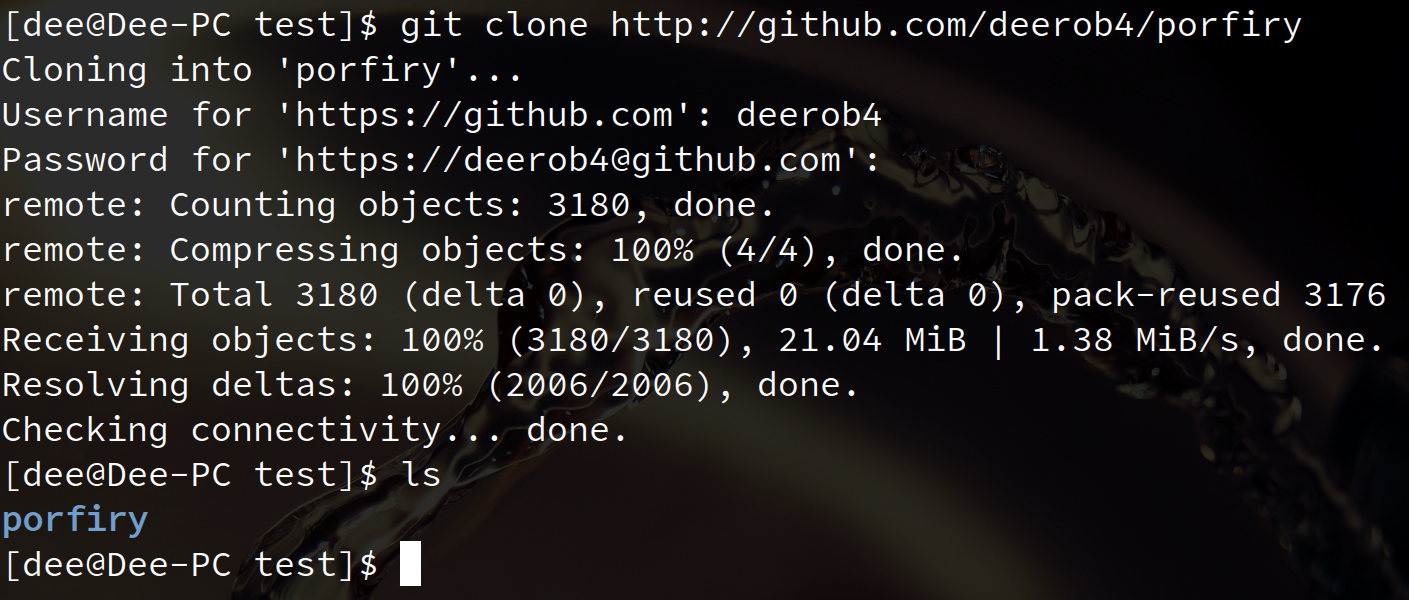
\includegraphics[scale=0.25]{user_guide/installation/clone}
  \caption{Cloning the repository.}
\end{figure}
% subsection cloning_the_repository (end)

\subsection{Installing Dependencies} % (fold)
\label{sub:installing_dependencies}
The next stage is to install the application's external dependencies. Without these, the system will not be able to run. Ensure that Node is installed on the server; if not, install it using the appropriate package manager. The minimum version of Node required is 4.2.3. To install the dependencies, run the following command:

\begin{verbatim}npm install\end{verbatim}

This will create an \textit{npm\_modules} directory in the root of the system's folder, which will contain all of the dependencies. The system will pull from this directory, so it is important that it is not moved.

\begin{figure}[h!]
  \centering
  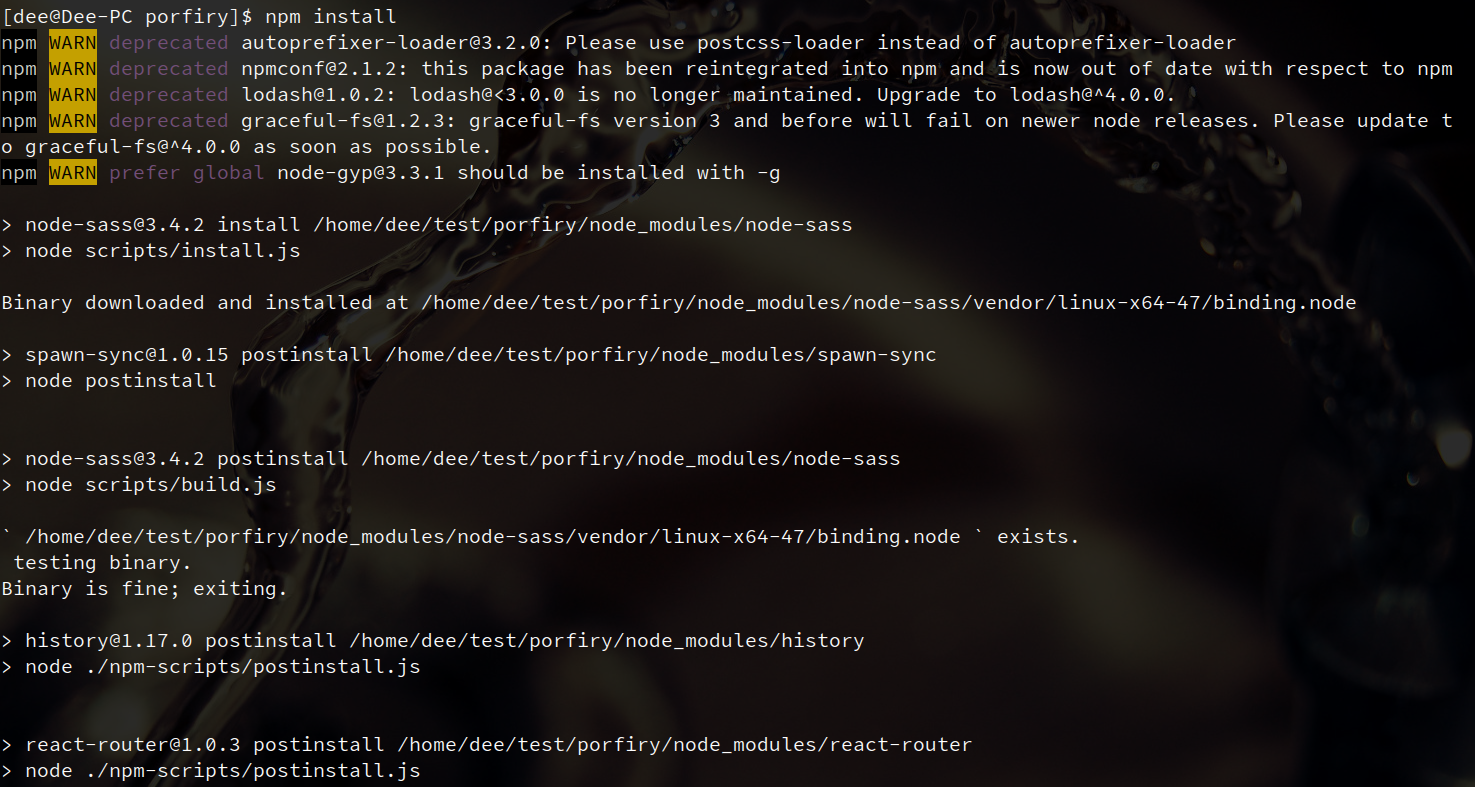
\includegraphics[scale=0.25]{user_guide/installation/deps}
  \caption{Installing the dependencies.}
\end{figure}
% subsection installing_dependencies (end)

\subsection{Starting the System} % (fold)
\label{sub:starting_the_system}
The final stage is actually starting the system. This is the easiest stage; simply type in:

\begin{verbatim}ENVIRONMENT=production npm start\end{verbatim}

This will start the server and all necessary sub-processes; it can then be left running. If for some reason the server needs to be switched off, any scheduled quizzes will still run next time it is turned on.

\begin{figure}[h!]
  \centering
  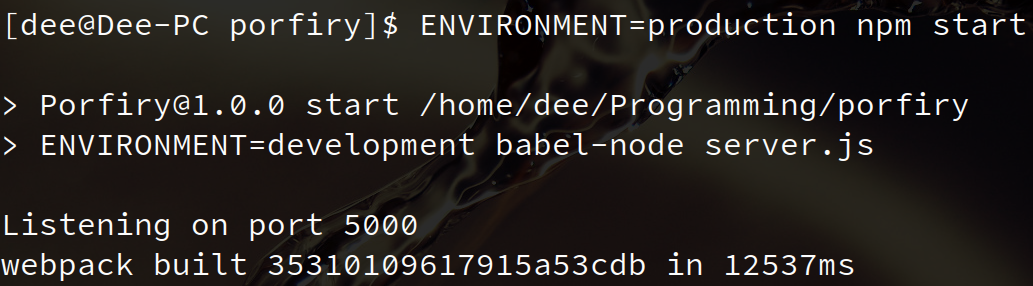
\includegraphics[scale=0.25]{user_guide/installation/start}
  \caption{Starting up the system.}
\end{figure}
% subsection starting_the_system (end)

% section installation (end)
